\chapter{MEM stage}
\label{chap:mem}

In this stage memory is read during a load and it is written during a store. Its block scheme is shown in figure \ref{fig:MEM_stage}.

\begin{figure}[!ht]
	\centering
	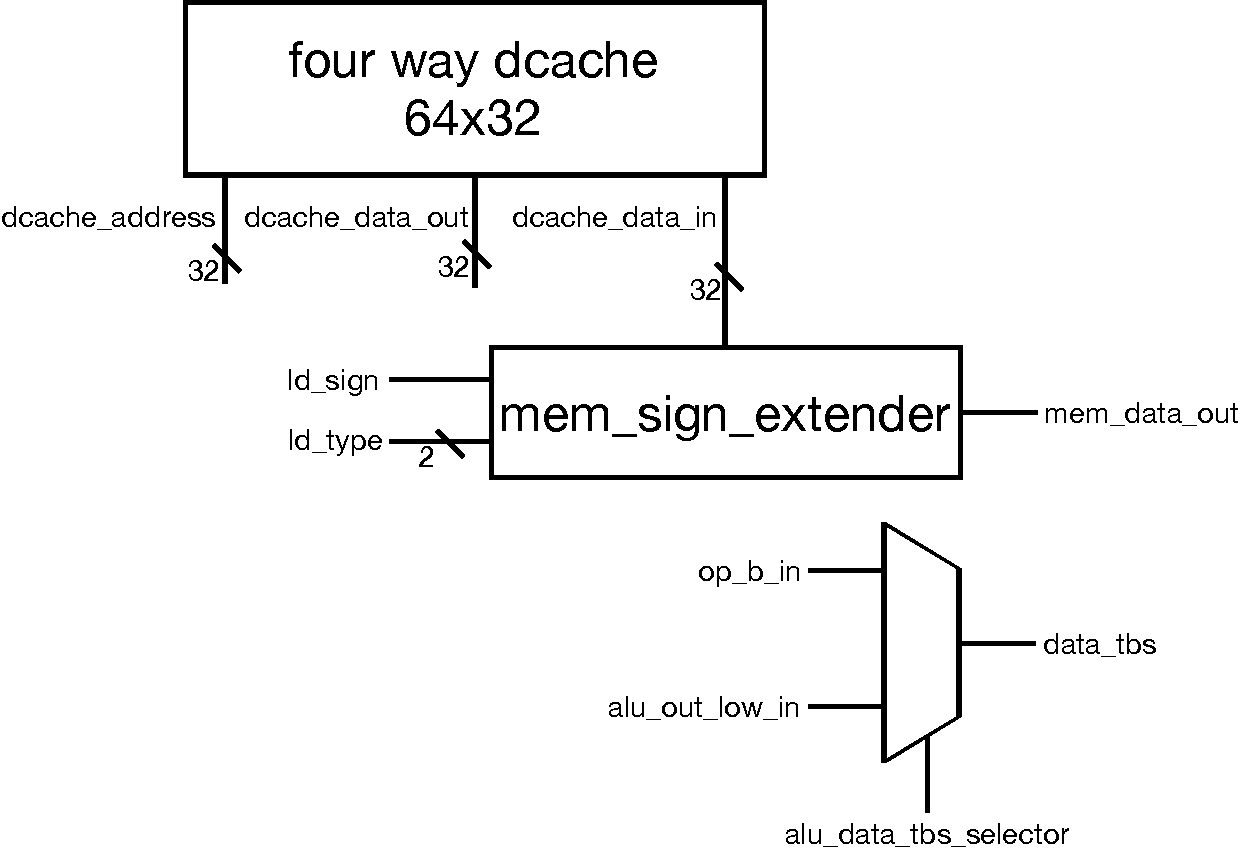
\includegraphics[width=.7\linewidth]{./chapters/figures/MEM_stage.pdf}
	\caption{Block diagram of the MEM stage}
	\label{fig:MEM_stage}
\end{figure}

The lowest mux is used when in the MEM stage when an operation different from a load and a store is executed. It selects \verb|alu_out_low_in| when in the RF the data coming from the ALU
must be stored, otherwise it selects \verb|op_b_in|, used by \verb|jalr| and \verb|jal| instruction to save in the RF the value of the program counter.

\section{Data cache}

The main datapath component of this stage is the data cache. It is a 64-entries four-way associative cache, able to perform two reads, two writes, or one read and one write per clock cycle.
This is due to the fact that the cache has two interfaces, one connected to the processor and another one connected to the memory controller. In figure \ref{fig:dcache} it is shown
the block diagram for the processor's side.

\begin{figure}[!ht]
	\centering
	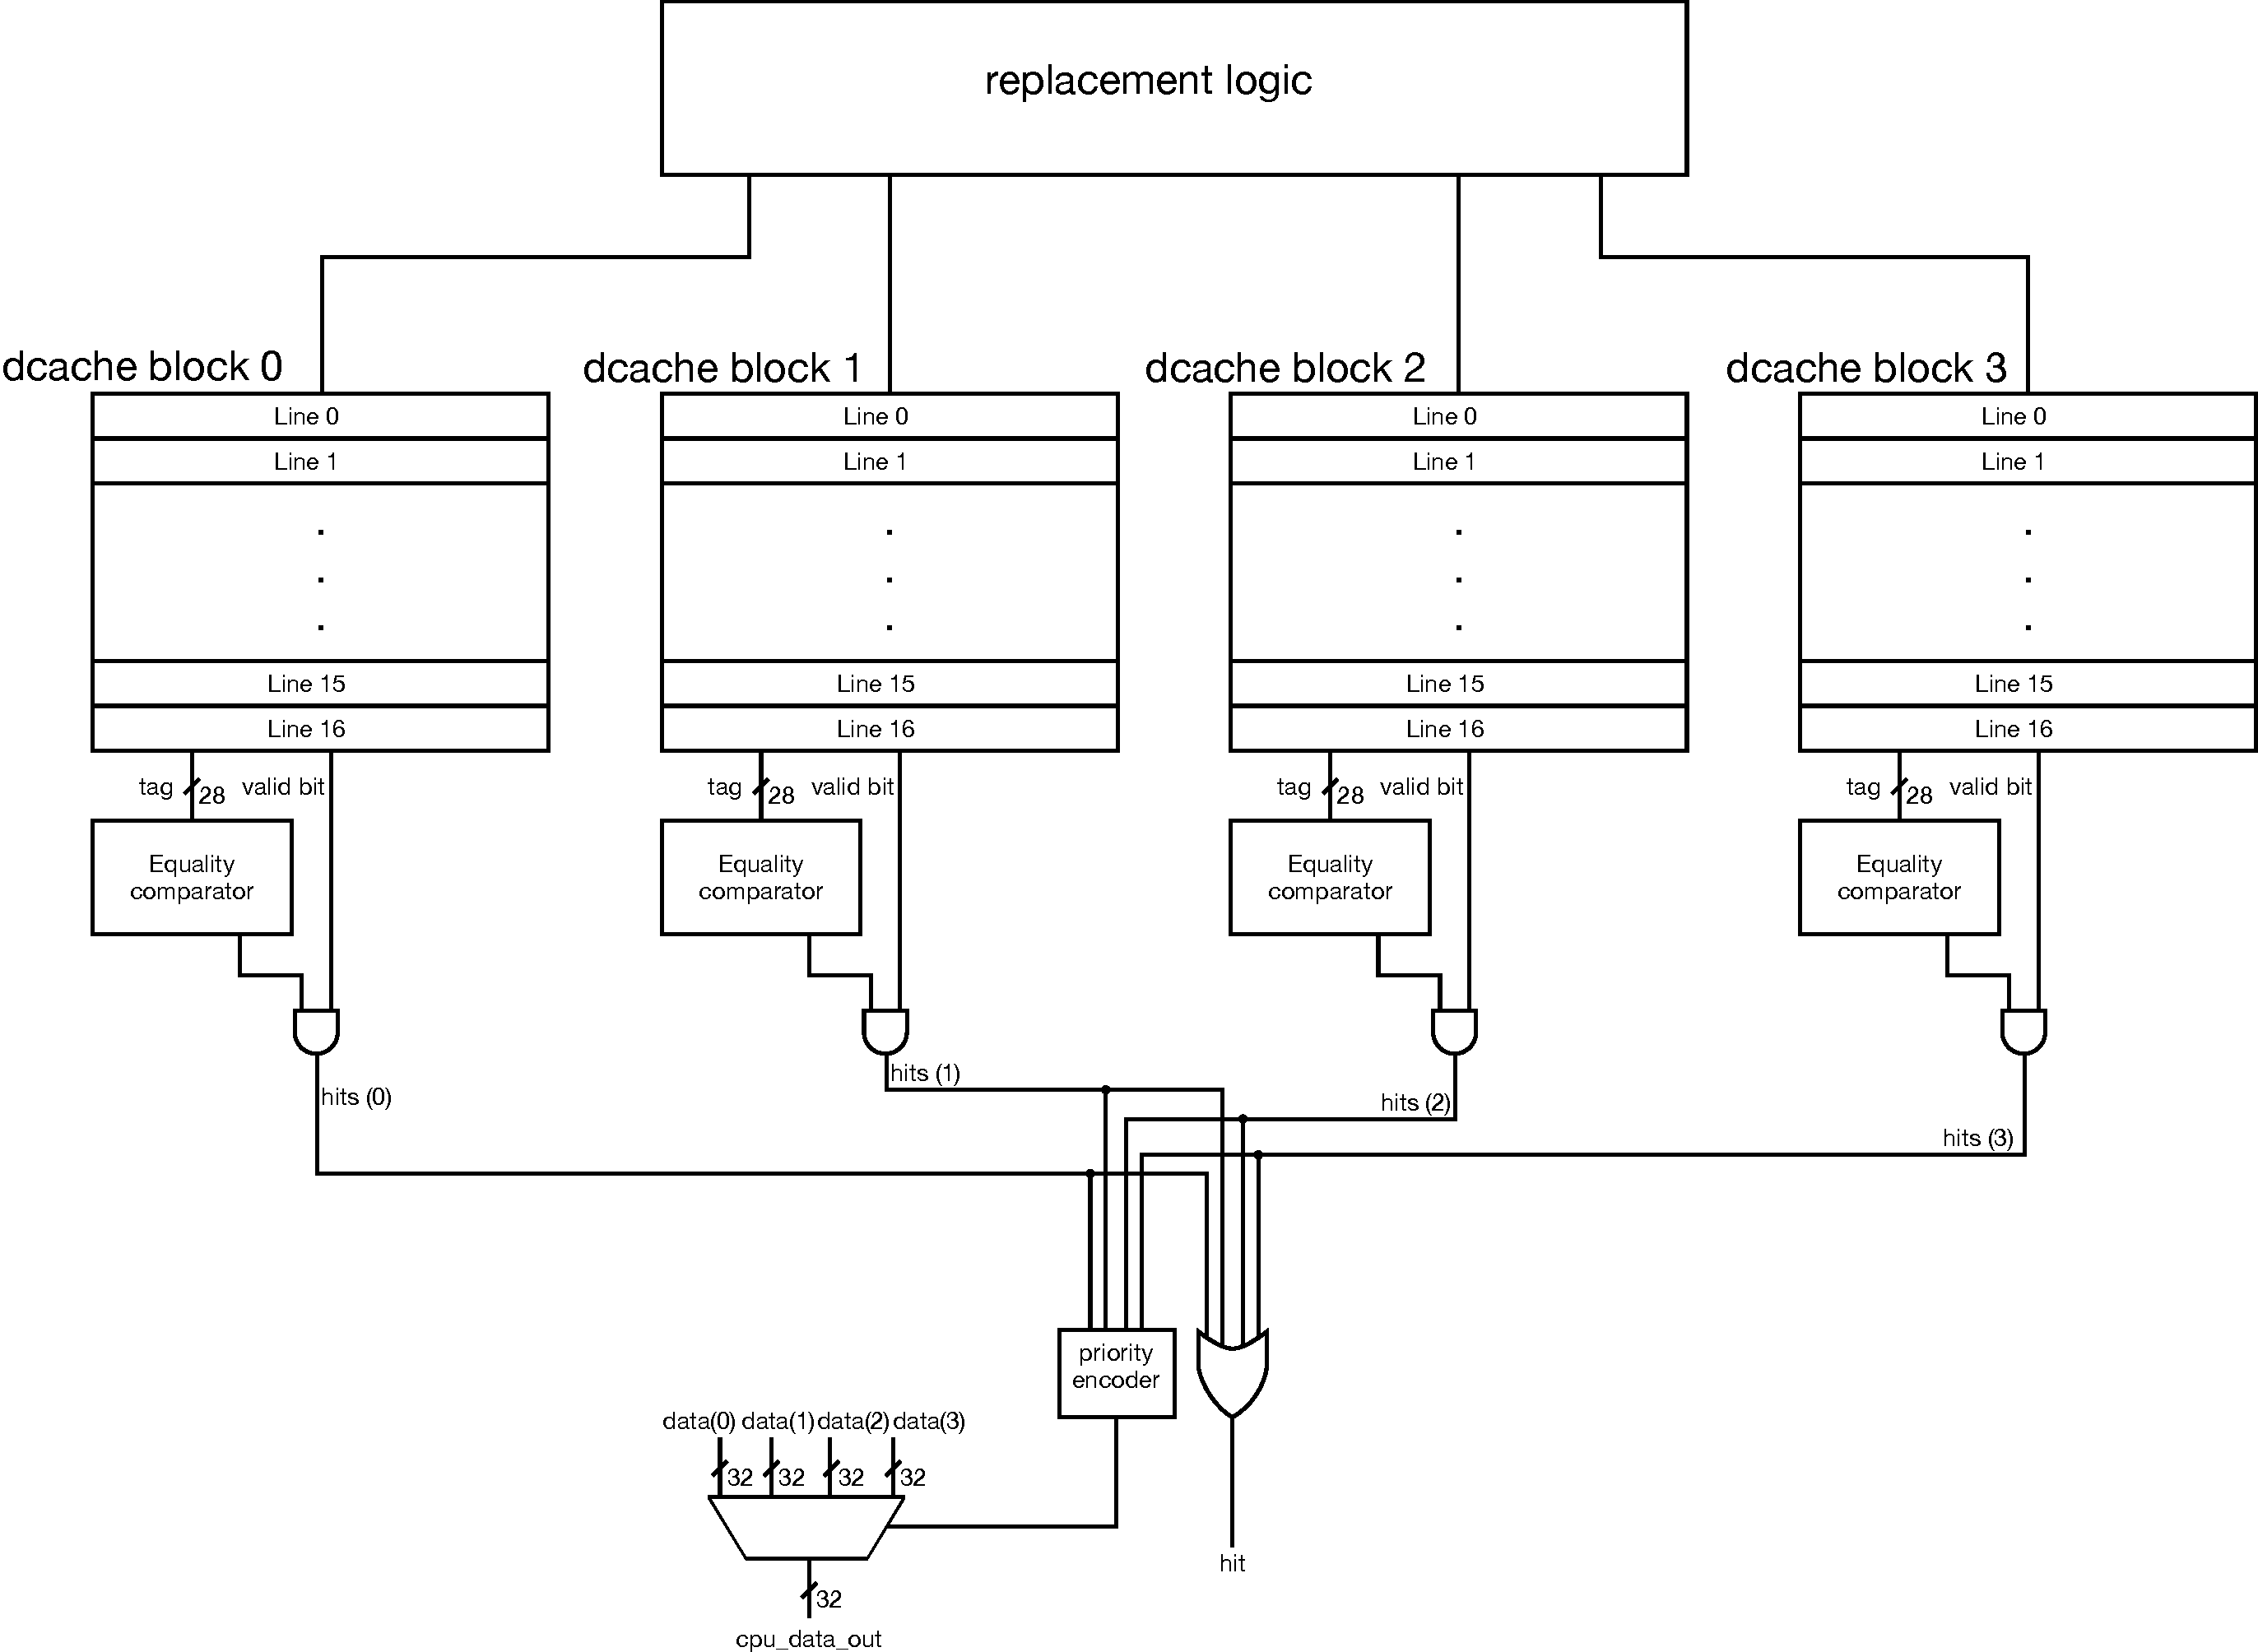
\includegraphics[width=\linewidth]{./chapters/figures/dcache.pdf}
	\caption{Dcache's processor side}
	\label{fig:dcache}
\end{figure}

As it can be seen, the cache's lines are divided among four blocks. Each line in a block corresponds to a different set, therefore a set is formed by considering all the lines having the same
number. The structure of the line is the same as the one shown in figure \ref{fig:BTB_cache_line}, but with a difference: if the data being stored comes from the CPU it is saved in big endian.
In fact, the DLX is expected to work in big endian, therefore every time data comes out the CPU it must do so in this format. To reuse some modules we already had, however, we preferred to internally
work in little endian. We've identified the cache as the best place to perform DLX-RAM data conversion transparently.

Moving on, each block has its own logic to detect if the line corresponding to the chosen set is generating a hit. The detection logic works in the same way as in the fully associative cache explained in section
\ref{subsec:fully_cache} and will not be discussed again. The four hits signal generated by the blocks then enter a priority encoder, which generate a suitable encoding for the data mux. Moreover, these signals
converge into a 4-inputs OR gate that outputs the final \verb|hit| signal.

\subsection{Replacement logic}

On top of the cache's blocks there is the replacement logic, shown in figure \ref{fig:dcache_replacement}.

\begin{figure}[!ht]
	\centering
	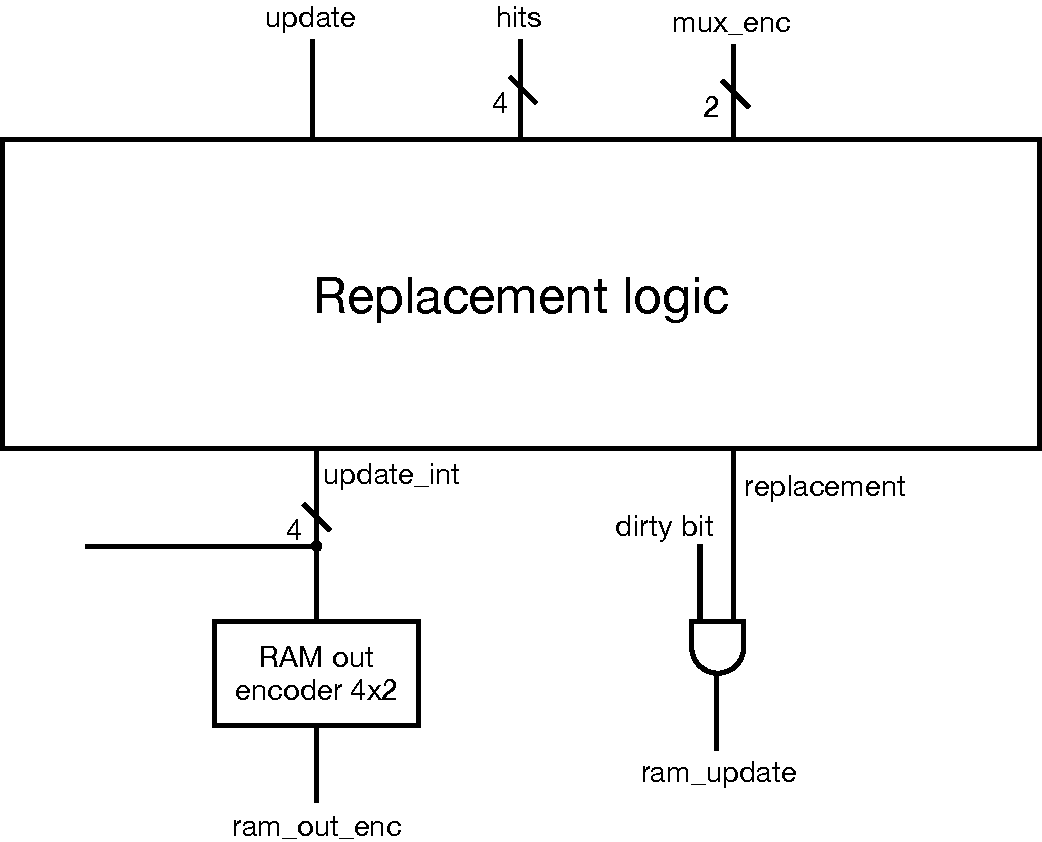
\includegraphics[width=0.6\linewidth]{./chapters/figures/dcache_replacement.pdf}
	\caption{Replacement logic}
	\label{fig:dcache_replacement}
\end{figure}

This unit receives in feedback the \verb|hits| signal generated by the four blocks and the encoding value for the data mux, moreover receives either from the memory controller or the control unit
an update signals. These information are combined together to decide how and if to update or replace the data contained in the cache.
When an update is requested for data not present yet in the cache and there are free blocks, a FIFO scheme is used and both \verb|replacement| and \verb|dirty_bit| are low.
On the other hand, when an update is requested for data already known to the cache, \verb|ram_out_enc| forwards the value of the input \verb|mux_enc| and it keeps \verb|replacement| low.
However, if new data must be written and there's no room in the blocks, an eviction must be performed. In this case the signal \verb|replacement| is raised to 1. Also the \verb|dirty_bit| is set to 1
since we are considering the case in which all the blocks are used. Hence, the AND goes to 1 and the both the control unit and the memory controller receive it.
For the explanation of how cache eviction and cache misses are handled please refer to section \ref{sec:cache_handling}.

\section{Sign extender}

The DLX, as seen in table \ref{tab:sup_instr}, supports many types of load operation: with or without sign extension, and on different sizes of data. The job of the sign extender is therefore the one
of taking in input the data read from the cache and to extend it properly (if necessary). It is driven by the control unit through the \verb|ld_sign| anf \verb|ld_type| signals. The former is set to 0
when load is unsigned, to 1 when it is signed. The latter is a 2-bit signals that specifies from where 0-extension or sign-extension should take place. The possible values are:

\begin{enumerate}
    \item \verb|00|: use 32 bits. In this case no operation is performed on the incoming data.
    \item \verb|01|:use 16 bits.
    \item \verb|10|: use 8 bits.
    \item \verb|11|: reserved. In this particular implementation it works in the same way as \verb|00|.
\end{enumerate}